%% ****** Start of file aiptemplate.tex ****** %
%%
%%   This file is part of the files in the distribution of AIP substyles for REVTeX4.
%%   Version 4.1 of 9 October 2009.
%%
%
% This is a template for producing documents for use with 
% the REVTEX 4.1 document class and the AIP substyles.
% 
% Copy this file to another name and then work on that file.
% That way, you always have this original template file to use.

%\documentclass[aip,graphicx]{revtex4-1}
%\documentclass[aip,reprint]{revtex4-1}

%\usepackage{graphicx}

%\draft % marks overfull lines with a black rule on the right
%\documentclass[pre,aps,floatfix,authordate1-4,twocolumn]{revtex4-1}
\documentclass[pre,aps,floatfix,authordate1-4]{revtex4-1}

%\documentclass[aps,prl,preprint,superscriptaddress]{revtex4}



%\documentclass[aps,prl,preprint,groupedaddress]{revtex4}

\usepackage{rotating} 
\usepackage{times}
\usepackage{graphicx}
\usepackage{setspace}
\usepackage{amsmath}
\usepackage{epstopdf}
\usepackage[obeyFinal]{easy-todo}
\begin{document}

% Use the \preprint command to place your local institutional report number 
% on the title page in preprint mode.
% Multiple \preprint commands are allowed.
%\preprint{}

\title{Rotational dynamics of proteins from spin relaxation rates and molecular dynamics simulations} %Title of paper

% repeat the \author .. \affiliation  etc. as needed
% \email, \thanks, \homepage, \altaffiliation all apply to the current author.
% Explanatory text should go in the []'s, 
% actual e-mail address or url should go in the {}'s for \email and \homepage.
% Please use the appropriate macro for the type of information

% \affiliation command applies to all authors since the last \affiliation command. 
% The \affiliation command should follow the other information.

\author{O. H. Samuli Ollila}
\email[]{samuli.ollila@helsinki.fi}
%\homepage[]{Your web page}
%\thanks{}
\altaffiliation{Department of Neuroscience and Biomedical Engineering, Aalto University}
\affiliation{Insititute of Biotechnology, University of Helsinki}

% Collaboration name, if desired (requires use of superscriptaddress option in \documentclass). 
% \noaffiliation is required (may also be used with the \author command).
%\collaboration{}
%\noaffiliation

\date{\today}

\begin{abstract}
  % insert abstract here
  
\end{abstract}

%\pacs{}% insert suggested PACS numbers in braces on next line

\maketitle %\maketitle must follow title, authors, abstract and \pacs

% Body of paper goes here. Use proper sectioning commands. 
% References should be done using the \cite, \ref, and \label commands


%\label{}

\section{Spin relaxation analysis from MD simulations}

Measurable spin relaxation rates are related to the molecular dynamics through
equations

...,

where $J(\omega)$ is the spectral density. The spectral density is the
fourier transformation of the second order rotational correlation function
for the bond under interest
\begin{equation}
  C(t)=\langle P_2(\theta) \rangle,
\end{equation}
where $P_2(\theta)=(3*\cos^2\theta-1)/2$ is the second order Legendre polynomial.
%and $\theta$ is the angle 
The rotational correlation function is often separated to overall and internal
motions of the molecule. Assuming that these are independent one can write
\begin{equation}
  C(t)=C_I(t)C_O(t),
\end{equation}
where $C_i(t)$ and $C_o(t)$ are correlation functions for internal and overall
rotiations, respectively. The internal correlation function decays to a plateau, which
is used to defined a order parameter respect to molecular axes $S^2$.
The internal correlation function can be then written by using
reduced correlation function $C'(t)$
\begin{equation}
  C(t)=[C'_I(t)(1-S^2)+S^2]C_O(t).
\end{equation}
The effective correlation time describing relaxation of internal
processes is then defined as
\begin{equation}
  \tau=\int_0^\infty g'(\tau) \mathrm{d}t.
\end{equation}
Fully anisotropic overall rotation can be described as a sum of five exponentials
\begin{equation}
  C_O(t)=\sum_{j=1}^5 A_j e^{-t/\tau_j},
\end{equation}
where
$\tau_1=(4D_{xx}+D_{yy}+D_{zz})^{-1}$,
$\tau_2=(D_{xx}+4D_{yy}+D_{zz})^{-1}$,
$\tau_3=(D_{xx}+D_{yy}+4D_{zz})^{-1}$,
$\tau_4=[6(D+(D^2-L^2)^{-1/2}]^{-1}$,
$\tau_5=[6(D-(D^2-L^2)^{-1/2}]^{-1}$,
$D=\frac{1}{3}(D_{xx}+D_{yy}+D_{zz})$ and 
$L^2=\frac{1}{3}(D_{xx}D_{yy}+D_{xx}D_{zz}+D_{yy}D_{zz})$.
The diffusion constants around
three principal axes of a molecule
$D_{xx}$, $D_{yy}$ and $D_{zz}$ are 
are defined as 
\begin{equation}
\begin{aligned}
  \langle (\Delta \alpha)^2 \rangle = 2 D_{xx} t \\
  \langle (\Delta \beta)^2 \rangle = 2 D_{yy} t \\
  \langle (\Delta \gamma)^2 \rangle = 2 D_{zz} t. \\
\end{aligned}
\end{equation}
%\begin{equation}
%  C'_I(t)= e^{-t/\tau_c},
%\end{equation}


Standard analyses of experimental relaxation data usually assume
fully or axially isotropic overall rotational motion and single
decay constant for interal motion. Then the free parameters
($S^2$, $\tau_j$, $A_j$) are fit against spin relaxation data
from experiments. This gives most likely very good results for
isotropic molecules for which the assumption of single internal
motional timescale is reasonable. However, for molecules with
significant shape anisotropy or several timescales in internal
motions the amoount parameters to be fitted becomes large compared
with the typical amount of experimental points.

On the other hand, trajectories of individual atoms can be calculated
from classical molecular dynamics simulations. The rotational
correlation functions can be calculated from such trajectories and
the internal and overall rotational motions can be explicitly
separated. If molecular dynamics simulation model reproduces
experimental spin relaxation rates, it can be used to interpret
the different dynamical processes present in the system.

An example of calculated rotational correlation function from
molecular dynamics simulation is shown in Fig.~\ref{exampleCORFF}.
Fourier transform of the total correlation function $g(t)$ gives
spectral density $J(\omega)$, which can be then embedded in Eqs. ??
to calculate the experimentally measurable spin relaxation rates.
If MD results agree with experiments, the simulation can be used
intepret the experimental data.
\begin{figure}[!h]
  \includegraphics[width=13cm]{../Figs/exampleCORRF.eps}%
  \caption{Example correlation functions from residue 269 of PsTonB simulated with OPC water model.
    Total correlation function $g(t)$ on (top). Correlation function for internal motions
    calculated from trajectory from which overall rotation of protein is removed.
    The plateau of this gives the order paramater square $S^2$.
    \label{exampleCORRF}}%
\end{figure}

The intertia tensor angles as a function of time and mean square angular
deviations are shown in Fig. \ref{exampleROTDIFFcalc}
\begin{figure}[!h]
  \includegraphics[width=18cm]{../Figs/exampleROTDIFFcalc.eps}%
  \caption{The intertia tensor angles as a function of time and mean square angular
    deviations for PsTonB simulation with OPC water model.
    \label{exampleROTDIFFcalc}}%
\end{figure}

The following steps are performed in practise. \\
1) Total rotational correlation functions $C(t)$ for protein N-H bonds are calculated from
MD simulation trajectory. The rotational correlation functions for internal dynamics $C_I(t)$ are
calculated from a trajectory from where the overall rotation of protein
is removed. The rotation is removed by using fit option in gmx trjconv and rotational
correlation functions are calculated with gmx rotacf. \\
2) The overall and internal motions are assumed independent. Overall
rotational correlation function can be then calculated from Eq. ref{??}
$C_O(t)=C(t)/C_I(t)$. \\
3) The protein axes of intertia and their root mean square deviations as function of
time are calculated from MD simulation trajectory. \\
4) Rotational diffusion constants $D_x$, $D_y$ and $D_z$ are calculated by fitting a straight line
to root mean square angle deviations of intertia axes. \\
5) The weighting factors $A_j$ are calculated by fitting Eqs. ref{??} in
rotational correlation functions of overall rotational motion $C_0(t)$. \\
6) The rotational diffusion constants are divided by the scaling factor and new
overall rotational correlation functions are calculated from Eq. ref {} by using
weights from previous step. New total correlation functions are calculated by
multiplying $C_I(t)$ from simulations with new overall correlation functions.

\section{Results and discussion}

The analysis method is demonstrated here for HpTonB short construct.
The calculated spin lattice relaxation times from simulations with different
water models together with experimental data \cite{??} are shown in Fig. \ref{relaxationDATAplot}.
The rotational diffusion constants for overall 

\begin{figure}[!h]
  \includegraphics[width=13cm]{../../TonB/Figs/relaxationDATAplot.eps}%
  \caption{Relaxation parameters for HpTonB short construct from
    experiments and simulations with Amber-ildn and different water models
    \label{relaxationDATAplot}}%
\end{figure}

\begin{table}[htb]
\centering
\caption{Rotational diffusion coefficients calculated directly from simulations in 303K.
  OPC RESULTS TO BE CHECKED.
}\label{ROTdiffCOEFFS}
\begin{tabular}{c c c c c c c }
  rad$^2$/ns   &    &  TIP3P  &   &   TIP4P   &  &   OPC \\
  \hline
  D$_{xx}$    &   &   0.083   &   &   0.038   &  &   0.030 \\
  D$_{yy}$   &    &  0.077   &    &   0.033   &  &   0.027 \\
  D$_{zz}$   &    &  0.16    &    &   0.059   &  &    0.058 \\
  2D$_{zz}$/(D$_{xx}$+D$_{yy}$) &  &   1.99    &  & 1.7    &	&  2.03 \\
  D$_{av}$  &    &   0.11    &    &   0.043   &  &   0.038 \\
  tau1     &  &  1.76	 &       &   4.13    &   &   4.87 \\
  tau2     &  &  1.82	 &       &   4.40    &   &   5.14 \\
  tau3     &  &  1.26	&        &   3.25    &   &   3.47 \\
  tau4     &  &  1.05	 &       &    2.75   &   &  2.94 \\
  tau5     &  &  3.05	 &       &    6.48   &   &   8.43 \\
  
  %\hline
\end{tabular}
\end{table} 

Results with rotational diffusion coefficient corrected with constant factor
are shown in Fig. \ref{relaxationDATAplotSCALED}. 
\begin{figure}[!h]
  \includegraphics[width=13cm]{../../TonB/Figs/relaxationDATAplotSCALED.eps}%
  \caption{Relaxation parameters for HpTonB short construct from
    experiments and simulations with Amber-ildn and different water models.
    The rotational diffusion coefficients are divided by 3.0 for tip3p simulation
    and by 1.3 for tip4p simulation.
    Experiments are done in 303K and simulations in 310K, simulations in 303K are running.
    \label{relaxationDATAplotSCALED}}%
\end{figure}

\begin{figure}[!h]
  \includegraphics[width=13cm]{../../TonB/Figs/relaxationDATAplotLONGERconstructSCALED.eps}%
  \caption{PRELIMINARY RESULTS for relaxation parameters for HpTonB longer construct (107) from
    experiments and simulations with Amber-ildn and tip4p water models.
    The rotational diffusion coefficients are divided by 1.3.
    Experiments and simulations are done in 303K.
    \label{relaxationDATAplotSCALEDlongerCONSTRUCT}}%
\end{figure}


\begin{table}[htb]
\centering
\caption{Rotational diffusion coefficients scaled with constant factor which
  gives a good agreement for spin relaxation data,  3.0 for tip3p simulation
    and by 1.3 for tip4p simulation.
  OPC RESULTS TO BE CHECKED.
}\label{ROTdiffCOEFFS}
\begin{tabular}{c c c c c c c }
  rad$^2$/ns   &    &  TIP3P  &   &   TIP4P \\%  &  &   OPC \\
  \hline
  D$_{xx}$    &   &   0.028   &   &   0.029 \\%  &  &   0.030 \\
  D$_{yy}$   &    &  0.026   &    &   0.025 \\%  &  &   0.027 \\
  D$_{zz}$   &    &  0.053    &    &   0.045 \\%   &  &    0.058 \\
  2D$_{zz}$/(D$_{xx}$+D$_{yy}$) &  &   1.99    &  & 1.7 \\%   &	&  2.03 \\
  D$_{av}$  &    &   0.034    &    &   0.033 \\%  &  &   0.038 \\
  %\hline
\end{tabular}
\end{table} 


\begin{table}[htb]
\centering
\caption{Rotational diffusion coefficients for different proteins based on MD analysis of NMR relaxation data
}\label{ROTdiffCOEFFS}
\begin{tabular}{c c c c c c c }
  rad$^2$/ns   &    &  HpTonB-92  &   & HpTonB-107  \\
  \hline
  D$_{xx}$    &   &   0.027 $\pm$ 0.001  &   &  0.020 $\pm$ 0.001 \\
  D$_{yy}$   &    &  0.027  $\pm$ 0.001  &    & 0.027 $\pm$ 0.001  \\
  D$_{zz}$   &    &  0.055   $\pm$ 0.005  &    &  0.050  $\pm$ 0.004 \\
  2D$_{zz}$/(D$_{xx}$+D$_{yy}$) &  &   2.0  $\pm$ 0.2    &  & 2.2   $\pm$ 0.1\\
  D$_{av}$  &    &   0.036  $\pm$ 0.003    &    &  0.033  $\pm$ 0.002  \\
  $\tau_{c}$(ns)  &    &  4.6   $\pm$ 0.4    &    &  5.1  $\pm$ 0.3 \\
  %\hline
\end{tabular}
\end{table} 


\newpage


\section{Results for PsTonB}

\begin{figure}[!h]
  \includegraphics[width=13cm]{../../PsTonB/Figs/relaxationDATAplotCOMP.eps}%
  \caption{Relaxation parameters for PsTonB short construct from
    experiments and simulations with Amber-ildn and different water models
    \label{hexPHASEdimensionsPLOT}}%
\end{figure}

\begin{table}[htb]
\centering
\caption{
}\label{ROTdiffCOEFFS}
\begin{tabular}{c c c c c}
rad$^2$/ns   &   &        TIP4P    &          &          OPC \\
D$_{xx}$ & &        0.026  & &         0.020 \\
D$_{yy}$  & &         0.022	 & &  0.022 \\
D$_{zz}$   & &       0.049	 & &  0.048 \\
D$_||$/D$_+$   & &   2.04	& &   2.31 \\
D$_{av}$    & &      0.03   & &       0.030 \\
tau1     & &     5.67	 & &         6.70 \\
tau2     & &     6.05	 & &         6.47 \\
tau3     & &     4.06	 & &         4.29 \\
tau4      & &    3.45	 & &         3.57 \\
tau5      & &    9.83	 & &         12.87 \\
  %\hline
\end{tabular}
\end{table}

\section{Results for Calmodulin}

\begin{figure}[!h]
  \includegraphics[width=13cm]{../../Calmodulin/Figs/relaxationDATAplot.eps}%
  \caption{Relaxation parameters for Calmodulin from
    experiments and simulations with Amber and CHARMM in tip3p
    \label{hexPHASEdimensionsPLOT}}%
\end{figure}

\begin{table}[htb]
\centering
\caption{ Overall rotational diffusion coeffiecents of Calmodulin from
  simulations by Pauline and hydrodynamical models with experimental data
  used by Barbato et al. \cite{barbato92}.
}\label{ROTdiffCOEFFS}
\begin{tabular}{c c c c c c c}
rad$^2$/ns &   &  AMBER & &  CHARMM & &  Hydrodynamics \\
D$_{xx}$ &     &  0.038  & &  0.033  & & 0.015 $\pm$ 0.5\\
D$_{yy}$  &    &  0.033  & &  0.034  & & 0.015 $\pm$ 0.5\\
D$_{zz}$   &   &  0.086  & &  0.065  & & 0.04 $\pm$ 1\\
D$_||$/D$_+$ & & 2.396	& &  1.96   & & 2.5 $\pm$ 0.3\\
D$_{av}$    &  & 0.053   & &  0.044  & & \\
tau1     &    & 3.66    & &  4.36   & & \\
tau2     &    & 3.88    & &  4.30   & & \\
tau3     &    & 2.40    & &  3.06   & & \\
tau4      &   & 2.05	& &  2.54   & & \\
tau5      &   & 6.91	& &  7.61   & & \\
  %\hline
\end{tabular}
\end{table} 

\begin{figure}[!h]
  \includegraphics[width=13cm]{../../Calmodulin/Figs/relaxationDATAplotREDUCEDrotation.eps}%
  \caption{Relaxation parameters for Calmodulin from
    experiments and simulations with Amber and CHARMM in tip3p.
    The overall rotation diffusion coefficiets are reduced to
    get better agreement with experimental spin relaxation times.
    \label{hexPHASEdimensionsPLOT}}%
\end{figure}

\begin{figure}[!h]
  \includegraphics[width=13cm]{../../Calmodulin/Figs/relaxationDATAplotNOIONS.eps}%
  \caption{Relaxation parameters for Ca2+ free Calmodulin from
    experiments \cite{tjandra95} \label{hexPHASEdimensionsPLOT}}%
\end{figure}

% If you have acknowledgments, this puts in the proper section head.
\begin{acknowledgments}
% Put your acknowledgments here.
%OHSO acknowledges Aalto science IT project and CSC-IT center for science for
%computational resources, and Emil Aaltonen foundation for funding.
\end{acknowledgments}

% Create the reference section using BibTe
\bibliography{refs.bib}

\newpage
\appendix
\begin{center}
{\bf SUPPLEMENTARY INFORMATION}
\end{center}


%\todolist
\end{document}
%
% ****** End of file aiptemplate.tex ******
